% =====================================================================
%  CIS 6270 Project 1 -- Group 2 -- Defense slides
%  BDG: Batch-Dispersion Guidance
%
%  Build:  pdflatex defense && pdflatex defense
%
%  RUBRIC COMPLIANCE BUILT IN:
%   * Every content slide carries its 1a-3e label in the TOP-RIGHT corner,
%     set by \lbl{...}.  The slides appear in order 1a -> 3e.
%   * On-slide numbered citations, with the matching source list in a very
%     small font at the BOTTOM-RIGHT, set by \srcs{...}.  Numbering restarts
%     on each slide, which the assignment permits.
%   * A Bibliography slide closes the deck.
%   * Figures are either original (ours) or carry a citation.
%
%  \TODO{...} marks a number the v3 run has not yet produced.
%  Speaker allocation is in slides/README_SLIDES.md, not on the slides,
%  because students may not use notes.
% =====================================================================
\documentclass[aspectratio=169,10pt]{beamer}

\usetheme{default}
\usecolortheme{default}
\setbeamertemplate{navigation symbols}{}
\setbeamertemplate{itemize items}[circle]
\setbeamercolor{frametitle}{fg=black}
\setbeamerfont{frametitle}{size=\large,series=\bfseries}

\usepackage[T1]{fontenc}
\usepackage[utf8]{inputenc}
\usepackage{booktabs}
\usepackage{amsmath,amssymb}
\usepackage{graphicx}
\usepackage{xcolor}
\usepackage{tikz}

\definecolor{accent}{HTML}{B3261E}
\definecolor{blue1}{HTML}{1F5FA9}
\definecolor{green1}{HTML}{2F6B4F}
\definecolor{grayt}{HTML}{6B6B6B}

% ---- the 1a-3e label, top right of every content slide ---------------------
\newcommand{\theslidelabel}{}
\newcommand{\lbl}[1]{\renewcommand{\theslidelabel}{#1}}
\setbeamertemplate{headline}{%
  \ifx\theslidelabel\empty\else
    \hfill\raisebox{-2.2ex}[0pt][0pt]{%
      \colorbox{accent!12}{\small\bfseries\color{accent}\,\theslidelabel\,}}\hspace{2.2ex}%
  \fi}

% ---- bottom-right source list, very small ----------------------------------
\newcommand{\srcs}[1]{\vfill{\raggedleft\color{grayt}\fontsize{4.9}{5.6}\selectfont #1\par}}

% ---- pending-number marker -------------------------------------------------
\newcommand{\TODO}[1]{\textcolor{accent}{\scriptsize[#1]}}

% ---- shorthands ------------------------------------------------------------
\newcommand{\Fbar}{\bar{F}}
\newcommand{\weff}{w_{\mathrm{eff}}}
\newcommand{\Vb}{V_{b}}
\newcommand{\ib}{\textsc{in-band}}
\newcommand{\take}[1]{\vspace{0.4ex}\colorbox{black!6}{\parbox{0.97\linewidth}{\footnotesize #1}}}

\title{\bfseries BDG: Batch-Dispersion Guidance for\\Property-Band Generation with Continuous Flow Matching}
\author{Bobo Li \and Henry Huang \and Idea Idehpour \and Haimo Fang}
\institute{CIS 6270, Group 2 \\ Department of Computer and Information Science, University of Pennsylvania}
\date{30 September 2026}

\begin{document}

% ============================== TITLE =======================================
{\lbl{}
\begin{frame}[plain]
  \titlepage
\end{frame}}

% ============================== 1a ==========================================
\lbl{1a}
\begin{frame}{Frame the study}
  \textbf{Problem.} Generate 3D molecules whose property lands inside a tolerance
  band around a target, without retraining the generator. A design campaign wants
  \emph{many usable candidates}, so the quantity that matters is \ib, the fraction of
  samples inside the band.

  \medskip
  \textbf{Central question.} Guidance concentrates a batch toward the target, and
  that dispersion is a by-product of its strength. Does making dispersion a quantity
  the user \emph{requests} raise band coverage?

  \medskip
  \textbf{Hypothesis.} At a centred target, coverage is limited by batch spread
  rather than centring error, so a calibrated spread setpoint should raise it.

  \medskip
  \textbf{Two continuous modalities.}
  \begin{itemize}\setlength\itemsep{0.15em}
    \item \textbf{Modality 1: QM9 3D molecular coordinates.} State space
      $\mathbb{R}^{N\times3}$ with a relaxed atom-type simplex, $N\le29$. Invariant
      to translation, rotation, atom permutation.
    \item \textbf{Modality 2: DNA enhancers on the probability simplex.} State space
      $(\Delta^3)^L$, one simplex per position over $\{$A,C,G,T$\}$. No rotation
      group; the constraint is that each position stays on the simplex.
  \end{itemize}

  \take{These are different state spaces, not two datasets of the same kind: one is
  a Euclidean coordinate space with a geometric group acting on it, the other a
  product of probability simplices.}

  \srcs{[1] Ramakrishnan et al. 2014 (QM9). [2] Hoogeboom et al. 2022 (EDM).
        [3] Tang et al. 2025 (MOG-DFM enhancer data).}
\end{frame}

% ============================== 1b ==========================================
\lbl{1b}
\begin{frame}{Data, splits, and leakage}
  \begin{columns}[T]
  \begin{column}{0.54\textwidth}
    \textbf{Modality 1: QM9} [1], pinned by SHA-256.\\
    133{,}885 molecules, explicit hydrogens.
    \smallskip

    {\small
    \begin{tabular}{llr}
      \toprule
      Split & Used for & $n$ \\
      \midrule
      \texttt{train\_a} & generator \emph{and} guide $f_A$ & 51{,}527 \\
      \texttt{train\_b} & evaluator $f_B$ only & 51{,}527 \\
      \texttt{val} & checkpoints, atom counts, $\delta$ & 17{,}748 \\
      \texttt{test} & held out & 13{,}083 \\
      \bottomrule
    \end{tabular}}
    \smallskip

    \textbf{How leakage is prevented.} $f_A$ and $f_B$ are trained on
    \emph{disjoint halves}, so the network that scores us never saw the data that
    trained the network that steers us. Normalisation constants come from
    \texttt{train\_a} alone. The calibration set that fixes $\delta$ is disjoint from
    the sets supplying targets and atom counts.
  \end{column}
  \begin{column}{0.44\textwidth}
    \textbf{Modality 2: Kenyon-cell enhancers} [3].\\
    6{,}126 \emph{Drosophila} sequences. The evaluator is an exact count, so no
    train/validation split is required and no leakage is possible.
    \smallskip

    \textbf{We do not merge the two species} distributed together. Their GC
    distributions differ, so steering spread on the mixture would partly steer the
    species mixing proportion, which is the quantity under study.
    \smallskip

    \textbf{Preprocessing.} Coordinates zero-centred per molecule, in \AA;
    dense $[B,29,\cdot]$ padding with a validity mask; DFT properties in
    D / Bohr$^3$ / Ha.
  \end{column}
  \end{columns}

  \srcs{[1] Ramakrishnan et al. 2014. [3] Tang et al. 2025.}
\end{frame}

\lbl{1b}
\begin{frame}{Representations, conditioning, modality-specific handling}
  \textbf{Representations, and why.}
  \begin{itemize}\setlength\itemsep{0.1em}
    \item \textbf{M1:} coordinates plus a \emph{relaxed} one-hot over
      $\{$H,C,N,O,F$\}$. Continuous relaxation is what lets one continuous flow
      carry both geometry and discrete types.
    \item \textbf{M2:} a point of $(\Delta^3)^L$ per sequence. The simplex is a
      continuous state space by the assignment's definition, and it is the native
      geometry of the sequence literature [4,5].
  \end{itemize}

  \medskip
  \textbf{Conditioning.} Base generation is \emph{unconditional}. The property
  enters only at sampling time through guidance. This is deliberate: a conditional
  model would give the controller nothing to steer and would break the M1/M2
  parallel we are testing.

  \medskip
  \textbf{Modality-specific handling.}
  \begin{itemize}\setlength\itemsep{0.1em}
    \item \textbf{M1 invariance:} translation by projection onto the
      zero-centre-of-mass subspace; rotation by messages depending only on squared
      pairwise distances with coordinate updates along difference vectors;
      permutation by symmetric pooling. Verified numerically, 12/12 gates to
      $\sim10^{-17}$.
    \item \textbf{M2 simplex mapping and decoding:} sequences are relaxed onto the
      simplex and decoded by per-position $\arg\max$; the property is scored by an
      \emph{exact} GC count on the decoded sequence.
  \end{itemize}

  \srcs{[4] Stark et al. 2024 (Dirichlet FM). [5] Davis et al. 2024 (Fisher Flow).}
\end{frame}

% ============================== 1c ==========================================
\lbl{1c}
\begin{frame}{Flow-matching baseline: mathematical formulation}
  Data $x_1\sim p_{\mathrm{data}}$, source $x_0$, time $t:0\to1$ from noise to data.

  \medskip
  \textbf{Probability path (linear interpolant)} [6]:
  \[ x_t = t\,x_1 + (1-t)\,x_0 ,\qquad
     u_t(x_t\mid x_0,x_1) = x_1 - x_0 \quad\text{(constant along the path)} \]

  \textbf{Source is not isotropic.} Coordinates are $x_0^{c}=\Pi_0\varepsilon$ with
  $\Pi_0$ the projection onto the zero-centre-of-mass subspace of the valid atoms,
  of dimension $3(N-1)$; type channels are a masked Gaussian.

  \medskip
  \textbf{Loss, exactly as implemented} (masked mean over valid entries, two heads
  normalised separately, $\lambda=1$):
  \[ \mathcal{L}_{\mathrm{FM}}(\theta)=\mathbb{E}_{t,x_0,x_1}\!\left[
     \tfrac{1}{3\Sigma M}\|M\odot(v^{c}_\theta-u^{c})\|^2
   + \lambda\tfrac{1}{K\Sigma M}\|M\odot(v^{f}_\theta-u^{f})\|^2\right] \]

  \textbf{New symbols.} $M$ atom mask, $K$ type channels, $v_\theta$ the learned
  velocity. Separate normalisation stops padding diluting the loss.

  \medskip
  \textbf{Endpoint estimate} that every guidance arm differentiates:
  $\;\hat{x}_1 = x_t + (1-t)\,v_\theta(x_t,t)$, available in closed form at every $t$.

  \srcs{[6] Lipman et al. 2022 (Flow Matching). [7] Liu et al. 2022 (Rectified Flow).
        [8] Albergo et al. 2025 (Stochastic Interpolants).}
\end{frame}

\lbl{1c}
\begin{frame}[shrink=15]{Flow-matching baseline: architecture, training, selection, sampling}
  \begin{columns}[T]
  \begin{column}{0.5\textwidth}
    \textbf{Architecture.} Dense E($n$)-equivariant graph network [9]: width 256,
    8 layers, SiLU, \textbf{3{,}753{,}229 parameters}. Time enters at the input
    embedding. No attention.
    \smallskip

    \textbf{Optimiser and schedule.} Adam, lr $2\times10^{-4}$,
    CosineAnnealingLR to 5\% of it, batch 256, gradient-norm clip 5.0, EMA decay
    0.9999 with warm-up. Sampling always uses the EMA copy.
    \smallskip

    \textbf{Budget.} 1500 epochs $=$ 303k steps, 11.4\,h on one B200 MIG slice,
    seed 20260918.
  \end{column}
  \begin{column}{0.5\textwidth}
    \textbf{Model selection (pre-registered).} Highest \emph{validation} atom
    stability at NFE 100, ties broken on validation loss, evaluated every 25 epochs.
    \smallskip

    \textbf{Disclosed amendment.} The rule selected epoch 1300; we ship epoch 1500,
    because the 512-sample selection signal could not resolve the last 200 epochs.
    The 3-seed $\times$ 10{,}000 benchmark confirms it on every metric
    ($+0.0018$ atom, $+0.0097$ molecule, $+0.0110$ validity, same sign on all seeds).
    \smallskip

    \textbf{Sampling.} Probability-flow ODE, \textbf{explicit Euler}, uniform grid,
    \textbf{100 steps $\Rightarrow$ NFE 100}. Quality saturates by 500 steps
    ($+0.65$ atom, $+2.8$ molecule from 100 to 500), so 100 is a cheap operating
    point.
  \end{column}
  \end{columns}

  \take{The closed-form endpoint estimate at every $t$ is the reason this family is
  convenient for guidance, and it is the property we use in 2a.}

  \srcs{[9] Satorras et al. 2021 (EGNN). [6] Lipman et al. 2022.}
\end{frame}

% ============================== 1d ==========================================
\lbl{1d}
\begin{frame}{Diffusion baseline: mathematical formulation}
  Continuous-time \textbf{variance-preserving} process [10,11], $\tau:0\to1$ from
  clean to noise, \textbf{linear} $\beta$:
  \[ \beta(\tau)=\beta_{\min}+\tau(\beta_{\max}-\beta_{\min}),\qquad
     \beta_{\min}=0.1,\;\beta_{\max}=20 \]
  \[ x_\tau=\alpha(\tau)x_0+\sigma(\tau)\epsilon,\qquad
     \log\alpha(\tau)=-\tfrac12\Big(\beta_{\min}\tau+\tfrac12(\beta_{\max}-\beta_{\min})\tau^2\Big),
     \qquad \alpha^2+\sigma^2=1 \]

  \textbf{Prediction target: $\epsilon$}, under the \emph{same} two-term masked-mean
  loss as the flow model, with coordinate noise projected onto the
  zero-centre-of-mass subspace so the target is equivariant. Times
  $\tau\sim\mathcal{U}(10^{-3},1)$ keep $\sigma$ away from zero.

  \medskip
  \textbf{Reverse sampler: probability-flow ODE}
  \[ \frac{\mathrm{d}x}{\mathrm{d}\tau}=-\tfrac12\beta(\tau)\big(x+s_\theta(x,\tau)\big),
     \qquad s_\theta=-\epsilon_\theta/\sigma \]
  integrated backwards on a decreasing 100-step grid, then a jump to the Tweedie
  posterior mean.

  \medskip
  \textbf{Derived quantities guidance consumes:}
  $\hat{x}_0=(x_\tau-\sigma\epsilon_\theta)/\alpha$ and $k=\sigma^2/\alpha$.
  Verified: $\alpha^2+\sigma^2=1$ to 6 d.p., $\alpha(0)=1$, $\alpha(1)=0.0066$.

  \srcs{[10] Song et al. 2021 (Score SDE). [11] Karras et al. 2022 (EDM).
        [2] Hoogeboom et al. 2022.}
\end{frame}

\lbl{1d}
\begin{frame}{Diffusion baseline: architecture, training, selection, sampling}
  \textbf{Matched by construction.} The diffusion baseline shares the
  representation, the split, the \emph{same EGNN backbone}, the optimiser, the
  learning-rate schedule, the batch size, the EMA, the gradient clipping, the seed
  and the \emph{same pre-registered selection rule} with the flow model. It differs
  \emph{only} in the corruption process. That is what makes 2a a comparison of
  families rather than of engineering.

  \medskip
  \begin{columns}[T]
  \begin{column}{0.5\textwidth}
    \textbf{Architecture and training.} EGNN 256$\times$8, 3.75\,M parameters,
    $\epsilon$-prediction head. Adam $2\times10^{-4}$, cosine to 5\%, batch 256,
    clip 5.0, EMA 0.9999, 1500 epochs.
    \smallskip

    \textbf{Model selection.} Highest validation atom stability at NFE 100, ties on
    loss, the identical rule.
  \end{column}
  \begin{column}{0.5\textwidth}
    \textbf{Sampling.} 100-step decreasing grid, then the Tweedie endpoint jump, so
    the unguided budget is \textbf{NFE 101} against the flow model's 100. We report
    that asymmetry rather than hiding it.
    \smallskip

    \textbf{Status, stated plainly.} Our own VP diffusion is implemented, gated and
    smoke-tested; the full-scale run is \TODO{v3 Job A}. The only \emph{measured}
    diffusion comparator today is a borrowed released checkpoint, and 2a labels it
    as such.
  \end{column}
  \end{columns}

  \take{We will not claim a family winner from a borrowed checkpoint. 2a states what
  the evidence does and does not support.}

  \srcs{[9] Satorras et al. 2021. [2] Hoogeboom et al. 2022. [11] Karras et al. 2022.}
\end{frame}

% ============================== 1e ==========================================
\lbl{1e}
\begin{frame}{Metrics: what we measure and what each one cannot tell us}
  \begin{columns}[T]
  \begin{column}{0.52\textwidth}
    \textbf{Control metric.}
    \begin{itemize}\setlength\itemsep{0.1em}
      \item \ib{} $=$ fraction of samples with
        $|f_B(x)-y|\le\delta$, scored by the \emph{held-out} evaluator.
      \item $\delta = 2\times f_B$'s calibration MAE on 3{,}000 molecules disjoint
        from the target and atom-count sets. \textbf{Pre-registered}, so it cannot
        be chosen after seeing results.
      \item Reported \emph{continuous and decoded}.
    \end{itemize}
    \smallskip
    \textbf{Decomposition.}
    $\mathrm{RMSE}^2=\mathrm{bias}^2+\mathrm{spread}^2$, both in units of $\delta$,
    plus spread relative to the unguided control. This is the quantity the
    innovation targets.
  \end{column}
  \begin{column}{0.48\textwidth}
    \textbf{Quality and diversity.} Atom stability, molecule stability, validity,
    uniqueness, novelty, pairwise diversity, under EDM conventions [2], with bond
    tables verified \emph{entry-for-entry} against the reference implementation.
    \smallskip

    \textbf{Sample counts.} Base models 3 seeds $\times$ 10{,}000. Guidance cells
    $n$ per cell $\times$ 3 seeds \TODO{v3 $n$}. Screening cells $n=256$--$512$,
    labelled wherever used.
    \smallskip

    \textbf{Limitation we state up front.} \ib{} rewards \emph{any} arm that
    contracts the batch, including onto chemically implausible structures. So every
    \ib{} number in this deck appears beside the chemistry it spent.
  \end{column}
  \end{columns}

  \take{No arm is ranked on \ib{} alone. A method that wins coverage by destroying
  molecules has not won.}

  \srcs{[2] Hoogeboom et al. 2022 (stability/validity conventions).}
\end{frame}

\lbl{1e}
\begin{frame}[shrink=15]{Fairness: what is matched, and what is not}
  {\small
  \begin{tabular}{lll}
    \toprule
    & \textbf{Matched} & \textbf{Disclosed mismatch} \\
    \midrule
    Data, split, preprocessing & identical & none \\
    Conditioning & unconditional both & none \\
    Atom-count distribution & drawn from \texttt{train\_a} both & none \\
    Evaluator, metric code, $\delta$ & identical & none \\
    Starting noise, seeds & shared, so arms are \emph{paired} & nothing paired \emph{across} backends \\
    Backbone & same EGNN 256$\times$8 & borrowed comparator is 256$\times$9 $+$ attention \\
    Parameters & 3.75\,M vs 3.75\,M & borrowed comparator 5.34\,M \\
    Sampling budget & 100 steps both & diffusion needs NFE 101 for its endpoint jump \\
    Training compute & identical recipe & \TODO{v3 Job A}; borrowed ckpt.\ budget unknown \\
    Feature scaling & ours unscaled one-hot & borrowed comparator scales by $1/4$ \\
    \bottomrule
  \end{tabular}}

  \medskip
  \textbf{Guidance-strength fairness.} The headline fixes $w=1$ for every arm. This
  asks \emph{what each rule does at one dial setting}, not which is best at its own
  optimum. \textbf{Equal $w$ is not equal force}: the measured applied-correction
  share spans $5.8\times$ across the arms where it can be measured, so every
  sentence quoting a headline number carries ``at $w=1$''.

  \medskip
  \textbf{Statistics.} Binomial standard errors; paired comparisons within a
  backend; multiplicity-corrected significance reported beside the single-test value
  because each arm is selected over a grid. \ib{} is \emph{never} compared across
  backends, because $\delta$ is set by that backend's evaluator.

  \srcs{Original table. Conventions from [2] Hoogeboom et al. 2022.}
\end{frame}

% ============================== 1f ==========================================
\lbl{1f}
\begin{frame}{Study overview}
  \centering
  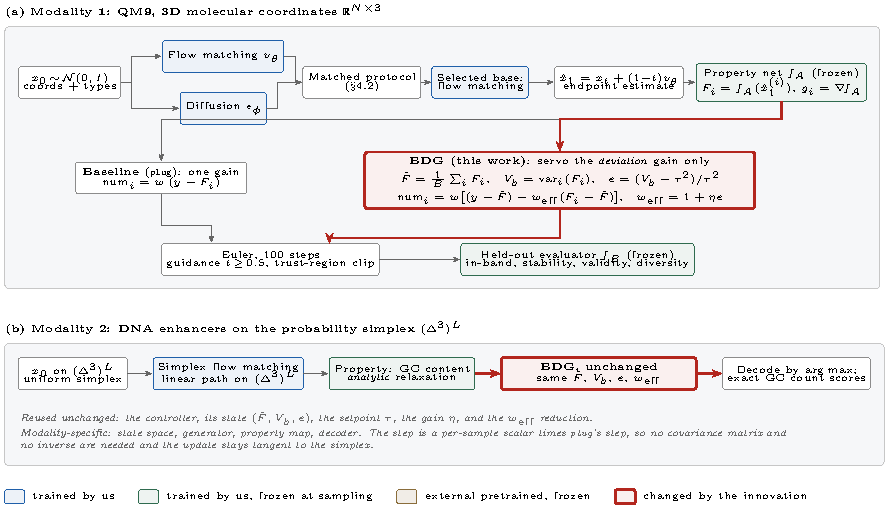
\includegraphics[width=0.86\linewidth]{../paper/figs/overview.pdf}

  \srcs{Original figure (this work). Components after [6] Lipman et al. 2022,
        [2] Hoogeboom et al. 2022, [4] Stark et al. 2024.}
\end{frame}

% ============================== 2a ==========================================
\lbl{2a}
\begin{frame}{Choose the base model}
  \centering
  {\small
  \begin{tabular}{llccccrr}
    \toprule
    Model & Source & Atom stab.$\uparrow$ & Mol.\ stab.$\uparrow$ & Validity$\uparrow$ & Uniq.$\uparrow$ & NFE$\downarrow$ & Params \\
    \midrule
    Flow matching (ours) & reproduced & $0.9366${\tiny$\pm.0012$} & $0.3993${\tiny$\pm.0085$} & $0.7625${\tiny$\pm.0031$} & $0.9939$ & $100$ & 3.75\,M \\
    VP diffusion (ours) & reproduced & \TODO{v3 A} & \TODO{v3 A} & \TODO{v3 A} & \TODO{} & $101$ & 3.75\,M \\
    \midrule
    \texttt{EDMsecond} [2] & borrowed ckpt. & $0.9644$ & $0.6725$ & $0.8490$ & \TODO{} & $100$ & 5.34\,M \\
    EDM, published [2] & quoted & $0.9870$ & $0.8200$ & $0.9190$ & $-$ & $1000$ & $-$ \\
    EDM, unscaled one-hot [2] & quoted & $0.9570$ & $0.4690$ & $-$ & $-$ & $1000$ & $-$ \\
    Real QM9 (ceiling) & measured & $0.9940$ & $0.9560$ & $0.9820$ & $1.0000$ & $-$ & $-$ \\
    \bottomrule
  \end{tabular}}

  \medskip
  \raggedright
  \textbf{Which model is carried forward, and why.} \textbf{Flow matching}, and the
  reason is \emph{not} a fidelity win. The matched own-diffusion row is
  \TODO{v3 Job A}, and the only measured diffusion comparator is a borrowed
  checkpoint that differs in architecture, training half and feature scaling, so it
  cannot decide the question. We carry flow matching because its linear path gives a
  \textbf{closed-form endpoint estimate at every $t$}, which is the object every
  guidance rule differentiates, at NFE 100 against a 1000-step published protocol.

  \smallskip
  \textbf{Our stability gap, attributed in rank order from our own measurements:}
  unscaled one-hot leads (the published ablation removing exactly that scaling costs
  3 atom / 35 molecule points); then training budget (303k steps vs $\approx$1.56M);
  half-data split \emph{ruled out} ($0.33$ atom points); evaluator \emph{ruled out}
  (bond tables match entry-for-entry).

  \srcs{[2] Hoogeboom et al. 2022 (EDM, Tables 1 and 10).}
\end{frame}

% ============================== 2b ==========================================
\lbl{2b}
\begin{frame}{Guidance strategy}
  \textbf{Rule and target.} A frozen property predictor $f_A$ is differentiated at
  the endpoint estimate $m_i$, and the gradient is pulled back to the sampling
  variable:
  \[ G_i=\frac{\mathrm{num}_i}{s^2}\,J_i^{\!\top}g_i ,\qquad
     \mathrm{num}_i^{\mathrm{plug}} = y-F_i ,\qquad
     F_i=f_A(m_i),\; g_i=\nabla_m f_A(m_i) \]
  Target $y$ is the \textbf{q50} value of the property, one fixed number per
  property. This is a DPS-style plug-in Gaussian-energy field [12].

  \medskip
  \begin{columns}[T]
  \begin{column}{0.5\textwidth}
    \textbf{Trained / pretrained / frozen.}
    \begin{itemize}\setlength\itemsep{0.05em}
      \item Generator $v_\theta$: trained by us, \textbf{frozen} at sampling.
      \item Guide $f_A$: trained by us on \texttt{train\_a}, \textbf{frozen},
        \texttt{eval()}, gradients disabled.
      \item Evaluator $f_B$: trained on \texttt{train\_b}, \textbf{frozen}, and it
        \emph{never participates in sampling}.
      \item Nothing is trained at guidance time.
    \end{itemize}
  \end{column}
  \begin{column}{0.5\textwidth}
    \textbf{Strength schedule, normalisation, clipping.}
    \begin{itemize}\setlength\itemsep{0.05em}
      \item Correction converted by $w(1-t)/t$.
      \item Denominator $s^2$ with $s=f_A$'s property standard deviation.
      \item \textbf{Velocity-relative trust region}: $G_i$ rescaled so
        $\|G_i\|\le\|v_i\|$, per sample, after $w$. Prior practice [13], shared by
        every arm.
      \item \textbf{Window:} guidance on for $t\ge0.5$ only.
    \end{itemize}
  \end{column}
  \end{columns}

  \take{The trust region is load-bearing, not cosmetic: removing it produces
  \textbf{222 non-finite samples} where the clipped run produces \textbf{0}.}

  \srcs{[12] Chung et al. 2023 (DPS). [13] trust-region practice, OSCAR-style.
        [14] Ho \& Salimans 2022 (CFG).}
\end{frame}

\lbl{2b}
\begin{frame}{Guidance works, and what it costs}
  \centering
  {\small
  \begin{tabular}{lccc}
    \toprule
    Arm & \ib$\uparrow$ & Spread\,/\,unguided & Mol.\ stab.$\uparrow$ \\
    \midrule
    unguided & $.090$\,/\,$.121$\,/\,$.051$ & $1.00$\,/\,$1.00$\,/\,$1.00$ & $.434$\,/\,$.434$\,/\,$.434$ \\
    plug-in (best $w$) & $.184$\,/\,$.219$\,/\,$\mathbf{.133}$ & $0.52$\,/\,$0.60$\,/\,$0.47$ & $.246$\,/\,$.199$\,/\,$.320$ \\
    TFG ($w{=}4$, $\mu$ only) [15] & $\mathbf{.535}$\,/\,$-$\,/\,$-$ & $0.22$\,/\,$-$\,/\,$-$ & $.172$\,/\,$-$\,/\,$-$ \\
    BDG ($w{=}32$, $\tau_{\mathrm{mult}}{=}0.5$) & $.180$\,/\,$\mathbf{.227}$\,/\,$.106$ & $0.49$\,/\,$0.68$\,/\,$0.53$ & $\mathbf{.348}$\,/\,$.262$\,/\,$.340$ \\
    \bottomrule
  \end{tabular}}

  \smallskip
  {\scriptsize Each cell is $\mu$\,/\,gap\,/\,$\alpha$. One generator, one seed,
  $n{=}256$, best strength per arm over $w\in\{0.05,\dots,32\}$, q50, no chemistry
  floor. Three-seed confirmation \TODO{v3}.}

  \medskip
  \raggedright
  \textbf{The target property improves.} $2.0\times$ on $\mu$, $1.9\times$ on the
  gap, $2.6\times$ on $\alpha$ for the plug-in rule; TFG reaches $6.0\times$ on
  $\mu$.

  \textbf{The cost is real and we report it.} Molecule stability falls from $0.434$
  unguided to $0.246$ (plug-in, $\mu$) and to $0.172$ (TFG). Validity falls with it.

  \textbf{The mechanism is visible.} Spread contracts from $1.00$ to $0.22$--$0.60$.
  Guidance works \emph{by concentrating the batch}, and the arm that contracts most
  wins \ib{} and loses the most chemistry.

  \take{That trade-off is inherited, not chosen. 2c asks whether the user can choose
  it instead.}

  \srcs{[15] Ye et al. 2024 (TFG). [12] Chung et al. 2023.}
\end{frame}

% ============================== 2c ==========================================
\lbl{2c}
\begin{frame}[shrink=15]{Motivate the innovation}
  \textbf{The weakness.} Coverage is a \emph{dispersion} problem at a centred
  target. Measured: guided batches sit $1$--$2$ band widths from the target while
  their spread is $5$--$9$ band widths. Yet every guidance rule optimises a
  \emph{centring} objective and exposes \emph{one} dial, $w$, which moves centring
  and spread together in a ratio the user never chooses.

  \medskip
  \textbf{The hypothesis.} If the sampler \emph{measures} its own batch dispersion
  and servoes toward a \emph{requested} value, the user trades spread against
  centring deliberately, in the units of the property rather than in units of push.

  \medskip
  \textbf{How this differs from prior work.} Each ingredient separately exists, and
  we claim none of them:
  {\small
  \begin{tabular}{ll}
    \toprule
    Prior art & What it already owns \\
    \midrule
    CFG-Ctrl [16], Feedback Guidance [17] & the guidance scale read as a control gain \\
    MGD [18] & empirical ensemble moments driven to a target, two-sided \\
    Variance-Tilted Diffusion [19] & batch spread targeting, widen-only, fixed linear feature \\
    Particle Guidance [20] & batch-coupled repulsion, no setpoint \\
    Negative-guidance window [21] & negative weight widens the distribution \\
    \bottomrule
  \end{tabular}}

  \medskip
  \textbf{What we did not find} in a bounded search (about eight queries, abstracts,
  25 Sep 2026): a scalar guidance weight set by the batch variance of a
  \emph{learned property predictor's own endpoint prediction}, against a
  \emph{two-sided user-chosen} setpoint, \emph{signed so the weight passes through
  zero}. That bounds our claim; it is not a priority claim.

  \srcs{[16] CFG-Ctrl arXiv:2603.03281. [17] FBG arXiv:2506.06085.
        [18] MGD arXiv:2602.17211. [19] VTD arXiv:2606.22239.
        [20] Corso et al. 2024. [21] Ventura et al. arXiv:2602.00716.}
\end{frame}

\lbl{2c}
\begin{frame}{Specify the innovation (1/2): the mechanism}
  \textbf{Two batch statistics and a scale-free error} (per guided step, batch $B$):
  \[ \Fbar=\tfrac1B\textstyle\sum_i F_i,\qquad
     \Vb=\tfrac{1}{B-1}\textstyle\sum_i(F_i-\Fbar)^2,\qquad
     e=\frac{\Vb-\tau^2}{\tau^2} \]
  \[ \boxed{\;\mathrm{num}_i=(y-F_i)-\eta\,e\,(F_i-\Fbar)
     \;=\;\underbrace{(y-\Fbar)}_{\text{centring, gain }w}
      -\underbrace{\weff}_{=\,1+\eta e}\,(F_i-\Fbar)\;} \]

  \begin{columns}[T]
  \begin{column}{0.5\textwidth}
    \textbf{A descent direction on the thing that binds.}
    $\partial\Vb/\partial F_i=\tfrac{2}{B-1}(F_i-\Fbar)$, and the chain rule carries
    it to $m_i$ along $g_i$. The $2/(B-1)$ is absorbed into $\eta$, so the gain does
    not scale with $B$.
    \smallskip

    \textbf{Signs are the whole mechanism.}
    $\Vb>\tau^2\Rightarrow$ contract; $\Vb<\tau^2\Rightarrow$ expand;
    $\Vb=\tau^2\Rightarrow$ the term vanishes and BDG is exactly the plug-in rule.
  \end{column}
  \begin{column}{0.5\textwidth}
    \textbf{Cost: zero extra NFE.} Both terms multiply the same $g_i$, so BDG shares
    the one backward pass the plug-in rule already performs. The cost accounting is
    byte-identical.
    \smallskip

    \textbf{Trainable: nothing.} The generator and $f_A$ stay frozen; only the
    sampler changes.
    \smallskip

    \textbf{New hyperparameters: two.} Gain $\eta$ and setpoint
    $\tau=\tau_{\mathrm{mult}}\cdot s$, reported as a fraction of the guide's own
    property standard deviation.
  \end{column}
  \end{columns}

  \srcs{Original formulation (this work). Plug-in base after [12] Chung et al. 2023.}
\end{frame}

\lbl{2c}
\begin{frame}{Specify the innovation (2/2): the reduction, and what bounds it}
  \textbf{We state the reduction ourselves.} $\mathrm{num}_i$ is affine in $F_i$, so
  it factors exactly:
  \[ (y-F_i)-\eta e\,(F_i-\Fbar)=\big(1+\eta e\big)\big(y_{\mathrm{eff}}-F_i\big),
     \qquad y_{\mathrm{eff}}=\frac{y+\eta e\,\Fbar}{1+\eta e} \]
  verified to $3.0\times10^{-15}$ analytically and $6.5\times10^{-7}$ on the real
  field.

  \medskip
  \begin{columns}[T]
  \begin{column}{0.52\textwidth}
    \textbf{What that means.} At any instant BDG is the \emph{plug-in field at a
    rescaled weight aiming at a shifted target}. It adds no new direction, and any
    guidance whose per-sample coefficient is affine in $F_i$ is the plug-in rule
    reweighted.
    \smallskip

    \textbf{What it does not remove.} $\weff$ is set \emph{online} from a measured
    quantity and may \emph{change sign}, which $w$ cannot do without also reversing
    the centring term.
  \end{column}
  \begin{column}{0.48\textwidth}
    \textbf{Bound.} $\Vb\ge0\Rightarrow e\ge-1\Rightarrow \weff\ge1-\eta$, for any
    batch. That bound licenses running two-sided with no clamp.
    \smallskip

    \textbf{Design constraint: $\eta>1$}, or $\weff$ never reaches negative values
    and the controller cannot expand at all.
    \smallskip

    \textbf{Equilibrium, stated honestly.} The law settles where $\weff=0$, that is
    $V^\star=\tau^2(1-1/\eta)$, an \emph{asymptote the 50-step window never reaches}.
    We therefore never say the controller holds its setpoint, and we order every
    table by \emph{measured} $\weff$.
  \end{column}
  \end{columns}

  \srcs{Original formulation (this work).}
\end{frame}

\lbl{2c}
\begin{frame}{The controller, measured}
  \centering
  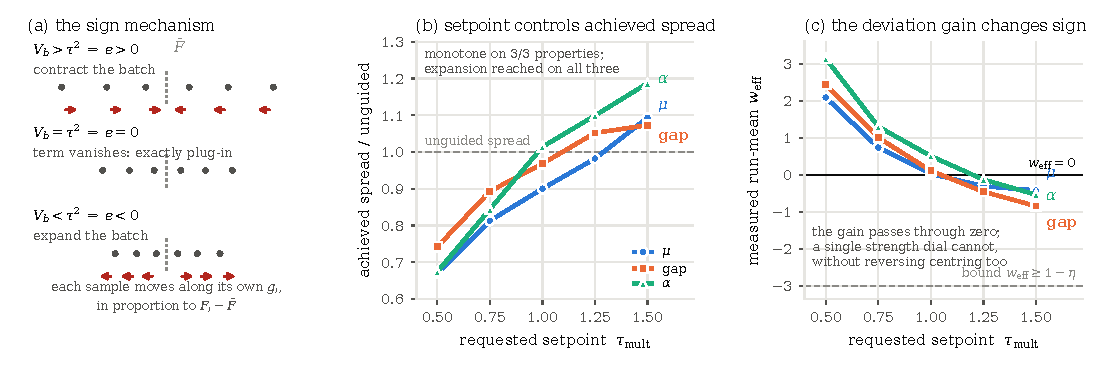
\includegraphics[width=0.98\linewidth]{../paper/figs/mechanism.pdf}

  \raggedright
  \footnotesize
  \textbf{(a)} The sign of $e$ is the whole mechanism, and $e=0$ recovers the
  plug-in rule exactly. \textbf{(b)} The requested setpoint maps monotonically onto
  achieved spread on \textbf{3/3} properties, and crosses \emph{above} the unguided
  spread on all three, which the strength dial does not reach. \textbf{(c)} The
  measured deviation gain \emph{passes through zero}, staying inside its bound
  $\weff\ge1-\eta$. A single strength dial cannot do that without reversing the
  centring term as well.

  \srcs{Original figure (this work), generated by
        \texttt{paper/figs/make\_mechanism.py} from
        \texttt{results/bdg\_port/table.txt} (64 cells, $n{=}256$, seed 20260925).}
\end{frame}

% ============================== 2d ==========================================
\lbl{2d}
\begin{frame}{Test the innovation: gates, ladder, controls}
  \centering
  {\small
  \begin{tabular}{llccccc}
    \toprule
    Variant & Role & $\eta$ & $\tau_{\mathrm{mult}}$ & Spread\,/\,ung. & \ib$\uparrow$ & Mol.\ stab.$\uparrow$ \\
    \midrule
    plug-in, $w{=}1$ & base & $-$ & $-$ & $0.714$ & $0.1094$ & $0.3633$ \\
    BDG $\eta{=}0$ & \emph{gate} & $0$ & $1.0$ & $0.714$ & $0.1094$ & $0.3633$ \\
    BDG one-sided, asked to expand & \emph{gate} & $4$ & $1.5$ & $0.714$ & $0.1094$ & $0.3633$ \\
    \midrule
    BDG contract & ladder & $4$ & $0.5$ & $0.670$ & $0.1406$ & $0.3359$ \\
    BDG neutral & ladder & $4$ & $1.0$ & $0.900$ & $0.0820$ & $0.4258$ \\
    BDG expand & ladder & $4$ & $1.5$ & $1.093$ & $0.0703$ & $0.4141$ \\
    \midrule
    plug-in, $w{=}4$ & \textbf{control} & $-$ & $-$ & $0.584$ & $0.1406$ & $0.2656$ \\
    open-loop $e$ replay, fresh noise & \textbf{control} & $4$ & $0.5$ & \multicolumn{3}{c}{recovers 69.5--96\% of the closed loop} \\
    signed-$w$ plug-in & \textbf{control} & $-$ & $-$ & \multicolumn{3}{c}{\TODO{not run; drop rule applies}} \\
    three-seed v3 grid & all & \multicolumn{4}{c}{\TODO{$\eta\in\{0,1,2,4,8\}\times\tau_{\mathrm{mult}}\in\{0.5,0.75,1,1.5\}$, $w\in\{1,4\}$}} \\
    \bottomrule
  \end{tabular}}

  \smallskip
  {\scriptsize Port cells, $n{=}256$, one seed, $w{=}1$, q50, own unguided control.
  Ladder ordered by \emph{measured} $\weff$, never by $\tau_{\mathrm{mult}}$.}

  \medskip
  \raggedright
  \textbf{Gates prove the implementation; they are not controls.} $\eta=0$ is
  bit-identical to the plug-in rule, so the dispersion term is the only addition. The
  one-sided variant asked to expand is also bit-identical (raw $e=-0.984$ clamped to
  $0$), so the sign branch is real and the clamp is self-consistently inert.

  \srcs{Original table (this work).}
\end{frame}

\lbl{2d}
\begin{frame}[shrink=15]{Conclusion from the ablations}
  \textbf{What each comparison isolates.}
  {\small
  \begin{tabular}{ll}
    \toprule
    Comparison & What it rules out \\
    \midrule
    $\eta=0$ vs plug-in & that anything other than the dispersion term changed \\
    one-sided vs two-sided & that the expansion branch is decorative \\
    the $\tau$ ladder & that the setpoint does not reach achieved spread \\
    plug-in at $w{=}4$ & that the coverage came from \emph{controlling} rather than \emph{pushing} \\
    open-loop $e$ replay & that the effect is feedback rather than a time-varying schedule \\
    signed-$w$ plug-in \TODO{} & that the same spread is not available more cheaply \\
    \bottomrule
  \end{tabular}}

  \medskip
  \textbf{What the evidence supports.}
  \begin{itemize}\setlength\itemsep{0.1em}
    \item \textbf{The setpoint controls spread}, monotonically, on \textbf{6 of 6}
      curves: $0.670\to1.219$ on the guide's scale, $0.650\to1.197$ on the
      evaluator's, reaching \emph{expansion above 1.0 on all six}, which the strength
      dial does not reach. $\weff$ changes sign up to \textbf{34 times} in the
      50-step window and spans $[-2.64,+10.35]$ against the bound $\weff\ge-3$.
    \item \textbf{Coverage does \emph{not} improve.} No rung beats plug-in at
      $|z|\ge3$: over \textbf{72 paired tests} the largest is $3.07$, which a
      \v{S}id\'ak correction turns into $p=0.14$. Removing the chemistry floor does
      not change this.
    \item \textbf{The trade-off, not the coverage, is what moves.} At \emph{matched}
      \ib{} of $0.1406$, BDG keeps molecule stability $0.3359$ against plug-in's
      $0.2656$.
  \end{itemize}

  \take{Honest reading: the schedule largely \emph{transfers} across seeds (69.5--96\%
  recovered open-loop) and feedback adds a small measurable remainder (0.3--6.6\%).
  We do \emph{not} claim the loop is irreducible to a schedule.}

  \srcs{Original analysis (this work).}
\end{frame}

% ============================== 2e ==========================================
\lbl{2e}
\begin{frame}{Position against recent work}
  \centering
  {\small
  \begin{tabular}{llcccrr}
    \toprule
    Method & Status & \ib$\uparrow$ & Mol.\ stab.$\uparrow$ & Diversity$\uparrow$ & Gen.\ passes & Guide passes \\
    \midrule
    DPS-style plug-in [12] & reproduced & \TODO{v3} & \TODO{v3} & \TODO{v3} & $10{,}000$ & $4{,}000$ \\
    TMPD-inspired [22] & reproduced & \TODO{v3} & \TODO{v3} & \TODO{v3} & $10{,}000$ & $4{,}000$ \\
    LGD-MC [23] & reproduced & \TODO{v3} & \TODO{v3} & \TODO{v3} & $12{,}000$ & $20{,}000$ \\
    TFG [15] & reproduced & \TODO{v3} & \TODO{v3} & \TODO{v3} & $8{,}000$ & $20{,}000$ \\
    D-Flow [24] & reproduced & \TODO{v3} & \TODO{v3} & \TODO{v3} & \TODO{} & \TODO{} \\
    \midrule
    Flow matching, unguided & internal ref. & \TODO{v3} & \TODO{v3} & \TODO{v3} & $10{,}000$ & $0$ \\
    \textbf{BDG (ours)} & reproduced & \TODO{v3} & \TODO{v3} & \TODO{v3} & $10{,}000$ & $4{,}000$ \\
    \bottomrule
  \end{tabular}}

  \smallskip
  \raggedright
  \textbf{Why these five.} All are inference-time guidance published in the last five
  years, all steer a frozen generator with a frozen predictor, and all run inside our
  pipeline on \emph{our} checkpoint. That isolates the \textbf{guidance rule} from the
  generator, which is what our contribution is about.

  \smallskip
  \textbf{Efficiency, measured not inferred.} BDG's two terms share one backward
  pass: \textbf{4{,}000} guide passes per cell against \textbf{20{,}000} for LGD-MC
  and TFG, a fifth of their guidance cost at the same generator budget. BDG is
  \emph{not} the cheapest overall: TFG uses fewer generator passes.

  \srcs{[12] Chung et al. 2023. [22] Boys et al. 2024 (TMPD).
        [23] Song et al. 2023 (LGD-MC). [15] Ye et al. 2024 (TFG).
        [24] Ben-Hamu et al. 2024 (D-Flow).}
\end{frame}

\lbl{2e}
\begin{frame}[shrink=15]{Fair study, and fair discussion}
  \textbf{Reproduced versus quoted.} Every row in the 2e table is
  \textbf{reproduced by us} on one frozen checkpoint, one guide, one evaluator, one
  target, one sample count. The only \emph{quoted} numbers anywhere in this study
  are the published base-model rows in 2a, and they are labelled as quoted and never
  pooled with ours.

  \medskip
  \textbf{Three port caveats we disclose rather than bury.}
  \begin{itemize}\setlength\itemsep{0.1em}
    \item Our plug-in arm is a \emph{DPS-style} Gaussian-energy field; the original
      DPS differentiates the residual $L_2$ norm [12].
    \item Our TMPD arm is the \emph{local-linear scalar limit} of the published
      method, included as a related-work comparison, not a faithful nonlinear
      port [22].
    \item TFG runs at its published QM9 hyperparameters but through \emph{our}
      deterministic ODE sampler, where the original used a stochastic DDIM update;
      our unscaled one-hot features also move $\approx16\times$ less relative to
      coordinates than the released checkpoint's. \textbf{These numbers must never be
      read against TFG's published table} [15].
  \end{itemize}

  \medskip
  \textbf{Where we are better, comparable, and worse.}
  \begin{itemize}\setlength\itemsep{0.1em}
    \item \textbf{Better:} chemistry retained at matched coverage; guidance cost, a
      fifth of LGD-MC's and TFG's guide passes.
    \item \textbf{Comparable:} \ib{} against the plug-in rule, which is the honest
      reading of the ablation null.
    \item \textbf{Worse:} TFG reaches far higher \ib{} ($0.535$ vs $0.180$ on $\mu$)
      at a chemistry cost we judge unacceptable ($0.172$ vs $0.348$), and it uses
      fewer generator passes. \TODO{v3 completes this comparison}
  \end{itemize}

  \srcs{[12] Chung et al. 2023. [22] Boys et al. 2024. [15] Ye et al. 2024.}
\end{frame}

% ============================== 3a ==========================================
\lbl{3a}
\begin{frame}{The transferred method}
  \begin{columns}[T]
  \begin{column}{0.5\textwidth}
    \textbf{What stays the same.} The \emph{whole controller}: $\Fbar$, $\Vb$, the
    error $e$, the setpoint $\tau$, the gain $\eta$, the bound $\weff\ge1-\eta$, and
    the reduction. \textbf{Transferred with zero code change.}
    \smallskip

    Why it can: BDG's step is a \emph{per-sample scalar} times the plug-in step, so
    it inherits that step's tangency and needs \textbf{no covariance matrix and no
    inverse}. That matters here, because the natural simplex covariance
    $\mathrm{diag}(p)-pp^{\!\top}$ is \emph{singular}.
  \end{column}
  \begin{column}{0.5\textwidth}
    \textbf{What must change.}
    \begin{itemize}\setlength\itemsep{0.05em}
      \item State space: $\mathbb{R}^{N\times3}\to(\Delta^3)^L$.
      \item Generator: EGNN $\to$ a linear-path flow model on the simplex.
      \item Property: a trained equivariant network $\to$ an \emph{analytic}
        differentiable relaxation of GC content.
      \item Evaluator: $f_B$ $\to$ an \emph{exact} GC count.
      \item Decoder: none $\to$ per-position $\arg\max$.
    \end{itemize}
  \end{column}
  \end{columns}

  \medskip
  \textbf{Training procedure (M2).} Linear-path flow matching on $(\Delta^3)^L$,
  trained on all 6{,}126 Kenyon-cell sequences, validation-based early stopping,
  checkpoint selected on validation loss. Architecture and budget: \TODO{v3 Job B}.

  \textbf{Sampling procedure (M2).} Same solver family and step count as M1, guidance
  applied on the same window, same velocity-relative trust region, decode by
  per-position $\arg\max$. The clip fired on \textbf{0--3\%} of steps, and the
  expanding cell clipped \textbf{once in 25{,}600}.

  \take{The transfer tests the \emph{controller}, not the property network. That is
  the point of changing the property from a learned net to an exact function.}

  \srcs{[3] Tang et al. 2025. [4] Stark et al. 2024. [5] Davis et al. 2024.}
\end{frame}

% ============================== 3b ==========================================
\lbl{3b}
\begin{frame}[shrink=15]{Transfer results}
  \centering
  {\small
  \begin{tabular}{lcc}
    \toprule
    Structural signature & QM9 & DNA simplex \\
    \midrule
    $\eta{=}0$ reproduces the plug-in rule & bit-identical & \textbf{bit-identical} \\
    one-sided at an expanding setpoint & exact & \textbf{exact}, $\weff{=}{+}1.000$ \\
    setpoint ladder monotone in spread & $0.67\to1.22$ & $0.81\to1.01$ \\
    cost identical to the plug-in rule & yes & \textbf{yes}, byte-identical \\
    contraction breaks the fidelity floor & yes & \textbf{yes} \\
    \ib{} improves & \textbf{no} & \textbf{no} \\
    \midrule
    \multicolumn{3}{l}{\emph{Against recent simplex sequence models, same protocol and sample count}}\\
    Dirichlet FM [4] & \multicolumn{2}{c}{\TODO{v3 Job B}} \\
    Fisher Flow [5] & \multicolumn{2}{c}{\TODO{v3 Job B}} \\
    MOG-DFM [3] & \multicolumn{2}{c}{\TODO{v3 Job B}} \\
    \textbf{BDG, transferred (ours)} & \multicolumn{2}{c}{\TODO{v3 Job B}} \\
    \bottomrule
  \end{tabular}}

  \medskip
  \raggedright
  \textbf{Fair study: this is not the published enhancer benchmark, and we say so.}
  The standard protocol is class-conditional generation at \textbf{500 bp} on
  81-class / 47-class sets of $\approx$90{,}000 sequences, scored by FBD over
  10{,}000 samples. We use \textbf{GC-band coverage}, \textbf{6{,}126} sequences and
  \textbf{200 bp}. Our base generator \emph{is} the linear-FM baseline these papers
  report, so it is a named baseline, but the numbers are not comparable and are never
  pooled.

  \smallskip
  \textbf{Three further disclosures.} Gumbel-Softmax FM does not run the enhancer
  benchmark at all, so only \emph{two} of the three closest named methods apply.
  Fisher Flow disputes the standard evaluator, reporting the cell-type classifiers
  behind it score \textbf{11.5\% / 11.2\%} test accuracy. MOG-DFM's own guided demo
  runs at length 100 while reporting base FBD at 500 bp.

  \srcs{[3] Tang et al. 2025. [4] Stark et al. 2024. [5] Davis et al. 2024.
        [25] Tang et al. 2025 (Gumbel-Softmax FM).}
\end{frame}

% ============================== 3c ==========================================
\lbl{3c}
\begin{frame}{Does the innovation transfer?}
  \textbf{Direction: yes, on every signature we can check.} The gates hold exactly,
  the ladder is monotone, expansion is reachable, the cost is unchanged, and the
  \emph{null} transfers too: spread control does not raise band coverage in either
  state space, and in both it is the \emph{contraction} rung that breaks the fidelity
  floor.

  \medskip
  \textbf{Magnitude: $2.6\times$ smaller}, a span of $0.20$ against $0.52$ in
  achieved spread. We attribute that to the \emph{property map}, not the controller,
  and we measured all three causes rather than assuming them:
  \begin{itemize}\setlength\itemsep{0.1em}
    \item \textbf{GC is affine} in the simplex coordinates, so its gradient is
      identical at every position and carries \emph{zero curvature}; the simplex
      renormalisation then partly undoes the edit.
    \item \textbf{GC is a 200-position average}, which suppresses the very variance
      the controller reads.
    \item \textbf{The band spans only $4.3$ attainable GC values} at granularity
      $1/200$. That is a ceiling on what \emph{any} method could move.
  \end{itemize}
  We ruled out the trust region: it fired on 0--3\% of steps, and the expanding cell
  clipped once in 25{,}600.

  \take{The evidence supports transfer of the \emph{mechanism and its limits}, and
  locates the magnitude difference in a measurable property of the task. The lever
  for a larger effect is a \emph{richer property}, for example a trained cell-type
  classifier logit, used as classifier \emph{guidance} rather than conditioning.}

  \srcs{Original analysis (this work).}
\end{frame}

% ============================== 3d ==========================================
\lbl{3d}
\begin{frame}{Limitations and failure modes}
  \textbf{1. The trust-region clip is a live confound at large $|\weff|$.}
  The plug-in rule clips on \textbf{884} sample steps where the contracting rung
  clips on \textbf{2{,}516}. At $\weff$ of order $10^3$ the dispersion term sits far
  outside the trust region, so what reaches the sample is the \emph{clip's
  truncation} of it. A rung can be \emph{clip-limited} rather than
  \emph{controller-limited}, and no metric in this study separates the two.
  \emph{Fix:} a run at matched clip activity.

  \medskip
  \textbf{2. The trade-off is re-parameterised, not removed.} The chemistry cost
  tracks $|\weff|$, not the \emph{direction} of the knob, so strongly contracting and
  strongly expanding rungs both cost chemistry. This is a descriptive correlation
  over coupled cells, not a test.

  \medskip
  \textbf{3. The batch is the estimator.} $\Vb$ is computed over whatever tensor the
  sampler is handed, so running $n$ samples in several batches runs \emph{several
  independent controllers}. Our headline batch of 500 is a memory constraint, not a
  modelling choice, and we disclose it wherever $n$ exceeds it.

  \medskip
  \textbf{4. The flow has a dispersion drift of its own.} The across-molecule
  variance \emph{contracts and then re-expands} on \emph{unguided} runs, so a
  setpoint on $\Vb$ is fighting a moving quantity.

  \take{Two of these are measured confounds, not speculation. They are the reason the
  controller claim is stated as provisional in 3e.}

  \srcs{Original analysis (this work).}
\end{frame}

% ============================== 3e ==========================================
\lbl{3e}
\begin{frame}[shrink=15]{Conclusion and future directions}
  \textbf{Back to the opening hypothesis.} We asked whether making batch dispersion
  a \emph{requested} quantity raises band coverage. \textbf{It does not}, and we can
  say why rather than only that.

  \medskip
  \textbf{The strongest conclusion the two-modality evidence supports.} Servoing the
  \emph{deviation} gain of a property-gradient guidance term against a
  batch-dispersion setpoint gives \textbf{monotone, two-sided, modality-portable}
  control of the generated batch's spread at \textbf{no additional sampling cost},
  and converts the coverage-against-fidelity trade-off into a quantity the user
  \emph{requests} rather than removing it.

  \medskip
  \textbf{Mechanism, and the trade-off.} The per-sample coefficient is
  \emph{affine} in $F_i$, so BDG is the plug-in field at a rescaled weight aiming at
  a shifted target: it cannot reach outside that field's reachable set. What it
  changes is \emph{which point} of that set the sampler lands on, and \emph{how} it
  gets there. Because the centring gain stays at $w$ while only the deviation gain is
  servoed, BDG buys contraction from the deviation mode rather than by scaling the
  whole field, which is why it retains more chemistry at matched coverage.

  \medskip
  \textbf{Specific next experiments.}
  \begin{itemize}\setlength\itemsep{0.05em}
    \item \textbf{The signed-$w$ plug-in control}, with our pre-registered drop rule:
      if it reaches BDG's spread at equal chemistry, we withdraw the controller claim
      and report the decomposition instead.
    \item \textbf{A matched-clip-activity run}, to separate clip-limited from
      controller-limited rungs.
    \item \textbf{A second seed pair} for the open-loop replay.
    \item \textbf{A richer M2 property} (cell-type classifier logit, nonlinear and
      motif-driven) to test whether the magnitude gap is the property map.
  \end{itemize}

  \srcs{Original conclusions (this work).}
\end{frame}

% ============================== BIBLIOGRAPHY =================================
\lbl{}
\begin{frame}{Bibliography (1/2)}
  {\scriptsize
  \begin{enumerate}\setlength\itemsep{0.05em}
    \item R.\ Ramakrishnan, P.\ Dral, M.\ Rupp, O.\ von Lilienfeld. Quantum chemistry structures and properties of 134 kilo molecules. \emph{Scientific Data}, 2014.
    \item E.\ Hoogeboom, V.\ Satorras, C.\ Vignac, M.\ Welling. Equivariant Diffusion for Molecule Generation in 3D. \emph{ICML}, 2022.
    \item T.\ Chen, Y.\ Zhang, S.\ Tang, P.\ Chatterjee. Multi-Objective-Guided Discrete Flow Matching. arXiv:2505.07086, 2025.
    \item H.\ Stark, B.\ Jing, C.\ Wang, G.\ Corso, B.\ Berger, R.\ Barzilay, T.\ Jaakkola. Dirichlet Flow Matching. arXiv:2402.05841, 2024.
    \item O.\ Davis, S.\ Kessler, M.\ Petrache, I.\ Ceylan, M.\ Bronstein, A.\ Bose. Fisher Flow Matching. \emph{NeurIPS}, 2024.
    \item Y.\ Lipman, R.\ Chen, H.\ Ben-Hamu, M.\ Nickel, M.\ Le. Flow Matching for Generative Modeling. arXiv:2210.02747, 2022.
    \item X.\ Liu, C.\ Gong, Q.\ Liu. Flow Straight and Fast: Rectified Flow. arXiv:2209.03003, 2022.
    \item M.\ Albergo, N.\ Boffi, E.\ Vanden-Eijnden. Stochastic Interpolants. \emph{JMLR}, 2025.
    \item V.\ Satorras, E.\ Hoogeboom, M.\ Welling. E($n$) Equivariant Graph Neural Networks. \emph{ICML}, 2021.
    \item Y.\ Song, J.\ Sohl-Dickstein, D.\ Kingma, A.\ Kumar, S.\ Ermon, B.\ Poole. Score-Based Generative Modeling through SDEs. \emph{ICLR}, 2021.
    \item T.\ Karras, M.\ Aittala, T.\ Aila, S.\ Laine. Elucidating the Design Space of Diffusion-Based Generative Models. \emph{NeurIPS}, 2022.
    \item H.\ Chung, J.\ Kim, M.\ McCann, M.\ Klasky, J.\ Ye. Diffusion Posterior Sampling. \emph{ICLR}, 2023.
    \item Velocity-relative trust region: adopted practice (see slide 2b); not claimed as ours.
  \end{enumerate}}
\end{frame}

\begin{frame}{Bibliography (2/2)}
  {\scriptsize
  \begin{enumerate}\setlength\itemsep{0.05em}\setcounter{enumi}{13}
    \item J.\ Ho, T.\ Salimans. Classifier-Free Diffusion Guidance. arXiv:2207.12598, 2022.
    \item H.\ Ye, H.\ Lin, J.\ Han, M.\ Xu, S.\ Liu, Y.\ Liang, J.\ Ma, J.\ Zou, S.\ Ermon. TFG: Unified Training-Free Guidance for Diffusion Models. \emph{NeurIPS}, 2024.
    \item CFG-Ctrl: classifier-free guidance as feedback control. arXiv:2603.03281, 2026.
    \item Feedback Guidance of Diffusion Models. arXiv:2506.06085, 2025.
    \item Moment Guided Diffusion. arXiv:2602.17211, 2026.
    \item Variance-Tilted Diffusion. arXiv:2606.22239, 2026.
    \item G.\ Corso, Y.\ Xu, V.\ De Bortoli, R.\ Barzilay, T.\ Jaakkola. Particle Guidance. \emph{ICLR}, 2024.
    \item E.\ Ventura, B.\ Achilli, L.\ Ambrogioni, C.\ Lucibello. Negative guidance reduces means and expands variances. arXiv:2602.00716, 2026.
    \item B.\ Boys, M.\ Girolami, J.\ Pidstrigach, S.\ Reich, A.\ Mosca, O.\ D.\ Akyildiz. Tweedie Moment Projected Diffusions. \emph{TMLR}, 2024.
    \item J.\ Song, Q.\ Zhang, H.\ Yin, M.\ Mardani, M.-Y.\ Liu, J.\ Kautz, Y.\ Chen, A.\ Vahdat. Loss-Guided Diffusion Models. \emph{ICML}, 2023.
    \item H.\ Ben-Hamu, O.\ Puny, I.\ Gat, B.\ Karrer, U.\ Singer, Y.\ Lipman. D-Flow: Differentiating through Flows for Controlled Generation. \emph{ICML}, 2024.
    \item S.\ Tang, Y.\ Zhang, A.\ Tong, P.\ Chatterjee. Gumbel-Softmax Flow Matching. arXiv:2503.17361, 2025.
  \end{enumerate}}
\end{frame}

\end{document}
